% Build this file; edit the manuscript's prose in chapter01.tex.
% The copied dissertation wrapper is preserved in main-dissertation.tex.bak.
\documentclass[12pt]{article}

% Page layout and the packages used by this manuscript.
\usepackage[margin=1in]{geometry}
\usepackage{graphicx}
\usepackage{mathtools}
\usepackage{enumitem}
\usepackage{array}
\usepackage{makecell}
\usepackage{tabularx}
\usepackage{hyphenat}
\usepackage{caption}
\usepackage{setspace}
\usepackage{sectsty}
\usepackage[most]{tcolorbox}
\usepackage{xurl}

% Keep the dissertation's APA citation style for this working draft.
\usepackage[american]{babel}
\usepackage{csquotes}
\usepackage[
  backend=biber,
  style=apa,
  language=auto,
  date=year,
  sorting=nyt,
  doi=false,
  isbn=false,
  url=false,
  maxcitenames=2,
  mincitenames=1
]{biblatex}
\DeclareLanguageMapping{american}{american-apa}
\addbibresource{references_v6.bib}
\AtEveryBibitem{\clearfield{note}}
\usepackage[hidelinks]{hyperref}

\doublespacing
\captionsetup{font=normalsize}
\sectionfont{\normalsize\bfseries}
\subsectionfont{\normalsize\bfseries}
\subsubsectionfont{\normalsize\bfseries}
\renewcommand{\arraystretch}{1.2}
\renewcommand\theadfont{\normalsize\bfseries}
\setlength{\extrarowheight}{2pt}
\graphicspath{{images/}}

% Working title and author, carried over from the dissertation.
\title{Modeling Group Misperceptions from Sampling and Perception-Mediated Dynamics}
\author{Vincent Wong, Yong-Yeol Ahn}
\date{}

\begin{document}
\maketitle

% Add the manuscript abstract here when it is ready:
% \begin{abstract}
% ...
% \end{abstract}

% !TEX root = main.tex
%====================================================
%  Abstract
%====================================================

% The first study is an agent-based model. The project is generally trying to model how ingroup and outgroup misperceptions happen, and it's doing so by trying to both answer generally yet-explored modeling of the non-motivated cognitive processes behind group misperception phenomena (pluralistic ignorance, false uniqueness, false consensus, etc) while situating itself in Self-Categorization Theory as a framework and trying to answer questions about how different aspects of that theory could play out if they're mechanically in opposition (like, what happens when ingroup members both conform to a perceived prototype while also separate their group identity from outgroups?). Bridging contributions to social psychology and network science.

%====================================================
%  Introduction
%====================================================

\section{Introduction}

% Overarching outline
% 1. Here's this problem: people misperceive the norms of groups that they voluntarily join. How does this happen? 
% 2. These social misperceptions have been found in these kinds of phenomena, and the findings are robust. 
% 3. The theory behind these mechanisms suggests that group categorization mental mechanisms are important (identity, norms, and intergroup contact)
% 4. These category-level mechanisms may not be sufficient to produce misperceptions if groups are dynamically configured to cause the effects to interact weirdly. Take Self-Categorization Theory (SCT) as an example: it predicts this and this. But these mechanisms suggest predictions but don't account for interrelated or configurational dynamics, like if people switch groups as group norms shift. 
% 5. Computational modeling is a great tool for studying group dynamics and group choice. Existing models tend to model interpersonal interactions rather than group categorization mechanisms, so there's an opportunity to study when these dynamics are mediated by group perceptions. 
% 6. In this paper, we present an agent-based model to test how misperceptions arise in dynamics of homophilic group choice when mediated by categorical group perceptions. 

%%% Introducing the problem
%%% People misperceive the norms of groups that they voluntarily join. How does this happen? 
People actively seek out social groups to join, whether for connection, shared interests, or a sense of belonging and identity. This enduring and earnest desire to connect with social groups is shown by contemporary online platforms like Meetup.com, Facebook groups, and niche online communities. 
Despite people's ability to freely socially affiliate, people still join and maintain membership in groups where they misperceive the prevailing consensus of the group. 
Undergraduates misperceive their own friends' attitudes towards substance use (\cite{prentice_pluralistic_1993}, \cite{amialchuk_influence_2019}), 
%  Prentice \& Miller,1993, Amialchuk/Ajilore/Egan 2018
members of vegetarian co-ops overestimate dietary stringency (\cite{kitts_egocentric_2003}), 
% Kitts, J. A. (2003). Egocentric bias or information management? Selective disclosure and the social roots of norm misperception. Social Psychology Quarterly, 222-237.
and people misperceive the extent of policy support in their own political party (\cite{ahler_parties_2018}). 
%Such mismatches between perception and reality can occur at the individual level, when members privately disagree with group norms, and at the collective level, when a majority misjudge the group's overall values. 
These phenomena present a broad puzzle: how could misperceptions persist even when people are directly motivated to seek out and join compatible groups?

%%% Covering the literature
%%% These social misperceptions have been found in these kinds of phenomena, and the findings are robust. 
Misperceptions of group behaviors, opinions, and norms have been found across a wide variety of social environments and at wildly different scales, including varying levels of voluntary association. 
At the level of ingroup misperception, this phenomenon is known as \emph{pluralistic ignorance}, which occurs when the people in a social group privately reject a norm but assume others accept it. For example, university students overestimate the extent to which their peers find cheating acceptable in relationships (\cite{boon_pluralistic_2014}), 
% Boon Watkins Sciban 2014
members of a small country experience pluralistic ignorance about their own opinions across a wide variety of political issues (\cite{shamir_pluralistic_1997}), and Americans underestimate the concern for climate change issues among other Americans (\cite{sparkman_americans_2022}). Another ingroup misperception phenomenon is \emph{false consensus}, where people believe that one's views are more widely shared in their group than they are. 
% ; and \emph{false uniqueness} is the opposite. 
Outgroup and intergroup misperceptions have also been documented, such as \emph{false polarization} 
where groups perceive themselves as more different from each other than they actually are. Groups may or may not experience both false polarization and varying levels of pluralistic ignorance simultaneously. 
These trends in misperceptions occur across scales, suggesting robust patterns even when people have different access to information about group members' attitudes, or when they know different subsets of their own group members.

%%% What mechanisms? 
%%% The theory behind these mechanisms suggests that group categorization mental mechanisms are important (identity, norms, and intergroup contact)
Existing social psychological research on these misperceptions proposes that people misperceive groups when they reason using their mental constructs about collectives of people, such as group norms, group identity, or the `typical' member. 
Social norms describe and prescribe expected or desired behaviors within a group, so they are a natural candidate for explaining misperceptions of group behaviors.
For example, first year undergraduates on US college campuses drink more than they personally feel comfortable with, with social norms around binge drinking as first years being a likely cause (\cite{borsari_drinking_2004}).
% Borsari 2003
People may also hold a concept of group identity which differs from the personal desires of the group's members. Homeless youth have been found to engage in more drug use than they prefer, and work suggests this may occur due to a desire to align with their group identity (\cite{barman-adhikari_descriptive_2017}). 
% Citations for PI and country-level cultural norms. 
Studies of pluralistic ignorance also suggest that people are affected by very broad mental constructs such as cultural norms. 
Work has found misperceptions of willingness to take paternity leave among Japanese men, and suggests this is influenced by Japanese gender narratives about men's contributions to familial life (\cite{miyajima_i_2017},\cite{kawamura_pluralistic_2024}). 
% Miyajima, T., & Yamaguchi, H. (2017). I want to but I won't: Pluralistic ignorance inhibits intentions to take paternity leave in Japan. Frontiers in Psychology, 8, 1508.
% Kawamura, Y., & Totake, K. (2024). Pluralistic ignorance did not prevent paternity leave in Japan in December 2021: A replication study. Japanese Psychological Research.


%%% Limitations of categorization-based theories
%%% These category-level mechanisms may not be sufficient to produce misperceptions if groups are dynamically configured to cause the effects to interact weirdly.
Although these explanations can account for particular aspects of these misperception phenomena, it is unclear if category-level mechanisms would interact to exacerbate or reduce group misperceptions in dynamically configured groups. One prominent overarching theory of group perceptions and identity, Self-Categorization Theory (SCT), explains how people form, perceive, and update group boundaries (\cite{turner_rediscovering_1987}). According to SCT, group perceptions shift under two major forces: (1) an internal attraction toward the prototypical ingroup member, where norms and perceptions gravitate toward the most representative members; and (2) a tendency to accentuate differences from outgroups, known as the meta-contrast principle. 
% While both verbal models make intuitive sense independently, they appear to conflict. Should perceptions converge toward the ingroup prototype, or diverge from relevant outgroups? Moreover, the notion of a ``prototypical group member'' is itself underspecified: does it refer to the numerical average of members, the person closest to current perceptions of the group, or the most extreme exemplar?
These two mechanisms may lead to the misperception of group norms if prototypical members are not representative of the group as a whole, or if the drive to differentiate from outgroups leads to exaggerated perceptions of ingroup opinions or identity.
However, as verbal models of human behavior, it is unclear if these two processes would interact and cancel each other out to produce accurate perceptions of groups. 

%%% Contribution of coputational models
%%% Computational modeling is a great tool for studying group dynamics and group choice. Existing models tend to model interpersonal interactions rather than group categorization mechanisms, so there's an opportunity to study when these dynamics are mediated by group perceptions. 
If the final outcome of group perception accuracy is dependent on configurational or dynamic factors, computational models are a strong tool to test how these mechanisms interact to produce different outcomes. 
%Computational modeling is a natural tool for testing how individual rules of group choice affect emergent group dynamics. 
Existing modeling work often focuses on representing publicly expressed opinions as a function of private opinions and aggregated dyadic interactions of others' public opinions, and showing how information flows on interpersonal network structures causing misalignment between private and public opinions. 
Research modeling pluralistic ignorance has found that it can arise through combinations of bounded confidence --- thresholds for agents to interact and exchange opinions --- and conformity rules between nearest neighbors on a lattice 
%Some research modeling pluralistic ignorance has found that it can arise through bounded confidence and conformity rules between nearest neighbors on a lattice 
(\cite{huang_novel_2014}). 
% https://jasss.soc.surrey.ac.uk/17/3/8.html
Other work focusing on modeling conformity (\cite{ye_influence_2019})
% https://www.sciencedirect.com/science/article/abs/pii/S0005109819302870
has found that kinetic models of networked opinion exchange (\cite{roy_opinion_2022}), 
% https://royalsocietypublishing.org/rsta/article/380/2224/20210169/112131/Opinion-dynamics-public-and-privateOpinion
and bounded confidence (\cite{hou_opinion_2021})
% https://www.sciencedirect.com/science/article/abs/pii/S0378437121002405
can produce phenomena where individuals privately disagree with what they publicly express.
Some work has found this to occur even at the local level of direct neighbors (\cite{manfredi_private-public_2020}). 
% https://journals.plos.org/plosone/article?id=10.1371/journal.pone.0242148

This existing work may not be able to account for the robustness of social norms which can persist even when observable evidence contradicts them. 
In order for these models of public and private opinion to represent group opinion, they commonly represent group norms as aggregate expressed opinion, leading them to conflate the two. 
Computational representations that focus on tracking group perceptions would allow us to test the effects of cognitive biases on these perception even when agents receive representative information about members' private opinions. 
This can also be a way to bridge the gap between verbal theories of group categorization and the dynamics of group misperception.

%%% Paragraph (Present research)
In this paper, we use agent-based modeling to test how misperceptions arise in dynamics of group choice when mediated by categorical group perceptions. 
We model agents which learn and update their perceptions of groups in the system, and decide which group to affiliate with based on the alignment between their private opinion and their perception of the group.
Group perceptions are treated as the primary perceptual unit where agents operate with individual perceptions of groups as coherent entities. 
This creates a coupled system where perceptions are dependent on group membership, and group membership is dependent on perceptions. 
Inspired by SCT, we implement competing mechanisms affecting these perceptions of groups, including a tendency to perceive groups as conforming to prototypical members and a tendency to perceive groups as distinct from one another.
We test how these mechanisms interact and produce different kinds of ingroup and intergroup misperceptions. 
This model formalizes and dynamically tests whether specific category-based inferential mechanisms are sufficient to generate particular macro-level misperception phenomena. 


%====================================================
%  Present work
%====================================================

\section{The present study}

% Description of this project
We use agent-based modeling to formalize individual-level mechanisms of perception change and to examine how they affect dynamics that produce misperceptions at the group level. In the model, agents hold both private opinions and perceptions of groups, and they seek to affiliate with the group that best aligns with their private opinions. When agents update their perceptions, they reconsider group membership based on their updated perception values. 
We implement alternative mechanisms for updating perceptions, drawn from Self-Categorization Theory, including (1) a tendency to drift toward prototypical ingroup members and (2) a tendency to drift away from outgroups. We further test different rules for defining prototypicality through sampling procedures. 

The model investigates how everyday processes of perception can generate persistent misalignments between perceived and actual group values, while also evaluating formalizations of SCT's mechanisms. In order to isolate the effect of perception change on model dynamics, agent private opinions remain fixed and all dynamics are driven by changes in their perceptions of groups. This allows us to test how the outcomes differ from similar agent-based models where personal opinion change is a driving factor. 

The central question is whether these known perception mechanisms can reproduce well\hyp{}documented misperception phenomena, such as pluralistic ignorance, in dynamic social contexts. We hypothesize that attraction alone produces persistent equilibrium misperceptions, whereas repulsion drives false polarization, with sampling rules modulating the prevalence of these outcomes.

%====================================================
%  METHOD
%====================================================

\section{Method}

We model a population of agents whose group affiliations and perceptions of social groups evolve over time. At each timestep, agents update their perceptions of each group based on sampled information from other agents, and then potentially revise their group membership based on the alignment between their own opinion and their perception of group norms. We then use this framework to test how changes in individual-level perception processes interact to produce population-level misperceptions of group norms.

The model consists of a number of fixed groups ($g \in \left\{ 1, \dots, K \right\}$) and $N$ individual agents, each of which belongs to one of the groups. Each agent has a private opinion and a perception of each group. Let $O_i$ be the private opinion of agent $i$ represented as a scalar, where $O_i \in [0,100]$. Agents' private opinions remain fixed throughout the simulation. 
Let $p_i(t)$ be a perception vector representing the agent $i$'s perception of each group in the system at time $t$, with components $p_{i,g}(t) \in [0,100]$ for each $g \in \left\{ 1, \dots, K \right\}$. Lastly, let $g_i(t)$ be the agent's group affiliation at time $t$, where $g_i(t) \in \left\{ 1 , \dots , K \right\}$. All dynamic behavior in the system arises from changes in agents' group memberships and group perceptions. 

The mechanism of group perception updating is motivated by Self-Categorization Theory (SCT, Turner et al., 1987), which emphasizes two forces shaping people's perceptions of groups: a pull toward prototypical ingroup members, and a push to accentuate differences between groups (the meta-contrast principle). From this, two mechanisms are operationalized into formal computational processes. First, we formalize the definition of a ``prototypical ingroup member'' as a sampling process where certain opinions are more likely to be seen than others. These sampling mechanisms specify how limited subsets of opinions become available to an agent at a given time. Second, we formalize how agents update their perceptions based on information about these members, including a pull toward prototypical members and a push to keep groups distinct. Conceptually, sampling governs the structure of informational exposure, whereas the update rules govern how agents cognitively integrate that information once observed.

We varied three sampling methods determining which group members' opinions are observed by an agent at each update. First, \textbf{proximity-biased sampling} selects opinions closer to an agent's current perception of a group. This mechanism can be interpreted as a form of confirmation bias, in which agents are more likely to encounter information consistent with their existing beliefs. 
This is consistent with self-categorization accounts in which prototypical group members are those perceived as congruent with the group norm. Second, \textbf{extremity-biased sampling} selects opinions with probability increasing in their distance from the center of the opinion scale, capturing the tendency for more extreme or salient opinions to be disproportionately visible due to social attention or media amplification (\cite{robertson_inside_2024}). 
Third, \textbf{random sampling} serves as a baseline where the opinions observed by the agent are representative of the group distribution. 

For the perception updating process, two mechanisms were implemented to test how their competing theoretical influences cause group misperceptions to arise. For the first perception updating rule, agents adjust their perceptions in response to direct evidence about other agents' private opinions obtained through sampling. In SCT, this is described as gaining information about prototypical group members, so we implement this as a tendency to allow values nearer to an agent's current perceptions to exert greater influence than values further away. 
We refer to this tendency in the model as Attraction, as it represents how agent perceptions shift toward available information.

Attraction is implemented computationally as follows: the agent takes the sample of private opinions and adjusts its perception value by shifting it toward those private opinion values. We use an updating rule with an exponential kernel that weights the changes in perception based on distance. This is specifically calculated as:

\[
p_{i,g}(t+1) \;=\; p_{i,g}(t) \;+\; \alpha \sum_{j \in S} \, (O_j - p_{i,g}(t)) \, e^{-\tfrac{|O_j - p_{i,g}(t)|}{\beta}}
\]

where \( p_{i,g}(t) \) is agent $i$'s perception of group $g$ at time $t$, $O_j$ is the opinion of group member $j$ from the set of sampled agent set $S$.~\( \alpha \) controls the amplitude of the effect (the amount of perception change per time step), and \( \beta \) controls the breadth of the effect (the rate of exponential decay). 

This form allows the rule to capture the SCT intuition that agents are pulled most strongly by information that is nearest their current perceptions of the group norm, i.e.~the group prototype. The exponential kernel is a common way of representing distance-decayed influence, where closer points of reference are weighted more heavily but distant ones are not ignored entirely. This form is structurally similar to gradient descent with an exponentially decayed, distance-dependent learning rate. In total, the Attraction effect causes agents' perceptions to shift more toward private opinion information that is more similar to their current perceptions.

The second perception updating mechanism is inspired by the meta-contrast principle from SCT, which states that people emphasize differences between the ingroup and outgroup in order to maintain sharper categorical boundaries. We implement this as a tendency for an agent's perceptions of groups to be shifted away from one another. The closer two perception values are, the stronger the repulsion force between them; conversely, perceptions that are already far apart are only weakly affected. We refer to this tendency as Repulsion.

Computationally, the Repulsion effect is defined analogously to Attraction but with the direction of influence reversed. Each perception value is pushed away from all other perception values held by the same agent, with the strength of repulsion weighted by an exponential-decay kernel. The update rule is:

\[
p_{i,g}(t+1) \;=\; p_{i,g}(t) \;+\; \gamma \sum_{k \neq g} \, \bigl(p_{i,g}(t) - p_{i,k}(t) \bigr)\,
e^{-\tfrac{|p_{i,g}^t - p_{i,k}^t|}{\eta}}
\]

where $p_{i,g}(t)$ is agent $i$'s perception of group $g$ at time $t$, and the summation runs over all other groups ($p_{i,k}(t), k \neq g$). The parameter $\gamma$ controls the amplitude of change (the rate of repulsion per time step), and $\eta$ controls the breadth of the exponential decay (how quickly the effect falls off with distance). Unlike Attraction, Repulsion only uses the agent's current perception values to calculate the updated perception values, and it does not sample or use private opinions in the calculation. 

At each timestep, $\delta$ (e.g., 100) agents are randomly selected to execute the following dynamics in order: (1) evaluate and update their perception of each group, and (2) choose whether to switch to another group based on homophily-driven updating. To update group perceptions, each agent samples private opinions of other agents and adjusts its perception value for each group based on that information, using specific update rules explained further below. To update group affiliations, agent $i$ evaluates its distance to its perception of each group and adopts the group for which this distance is minimized as

\[
g_i(t+1) = \arg \min_{g \in \left\{ 1, \dots, K \right\}} \| p_{i,g}(t) - O_i \|
\]

In summary, the model captures an intuition 
Perceptions drift over time as individual agents receive samples of information from both groups (Attraction). 
While this veracity-driven estimation process is occurring, agent's perceptions of groups are being pushed away from each other as agents attempt to keep their mental representations of each group distinct (Repulsion). 
As long as any change in perception is enough to lead an agent to perceive a different group as closer to them than their current group, the agent will switch to the other group. 
The effect of Attraction may lead agents to leave their current group as they obtain information about the outgroup. 
Below is a box containing the pseudo-code representing the complete algorithm for the model. 

% \begin{tcolorbox}[title=\textbf{[Simulation method]}, colback=white, colframe=black]
% \begin{itemize}[left=1em]
%     \item \textbf{Initialize:}
%     \begin{itemize}
%         \item Assign agents a private opinion as a random number between 0 and 100
%         \item Assign agents an initial group affiliation randomly; create edge
%         \item Assign each agents's perception of each group as a random number between 0 and 100
%     \end{itemize}
%     \item \textbf{For \( t \) in \textit{timesteps}:}
%     \begin{itemize}
%         \item Randomly select \( \delta \) number of agents to update
%         \item For each agent to update:
%         \begin{itemize}
%             \item[]\textbullet\ \ Sample \( \xi_{ingroup} \) number of ingroup members and \( \xi_{outgroup} \) number of outgroup members according to sampling rule
%             \item[]\textbullet\ \ Calculate and update perception values according to Attraction and Repulsion rules
%             \item[]\textbullet\ \ Update group affiliation to nearest group, according to perceptions
%         \end{itemize}
%     \end{itemize}
% \end{itemize}
% \end{tcolorbox}

\begin{tcolorbox}[title=\textbf{Simulation procedure}, colback=white, colframe=black]
\begin{itemize}[left=1em]
    \item \textbf{Initialize:}
    \begin{itemize}
        \item For each agent \(i\), assign a continuous-valued private opinion \(O_i \sim \text{Uniform}(0,100)\)
        \item For each agent \(i\), assign an initial group affiliation \(g_i(0)\) uniformly at random from \(\{1,\dots,K\}\)
        \item For each agent \(i\) and group \(g\), assign an initial integer-valued perception value \(p_{i,g}(0) \sim \text{Uniform}(0,100)\)
    \end{itemize}

    \item \textbf{For each timestep \(t = 0,1,\dots,T-1\):}
    \begin{itemize}
        \item Randomly select \(\delta\) agents to update
        \item For each selected agent \(i\):
        \begin{itemize}
            \item Sample \(\xi_{\text{in}}\) ingroup members and \(\xi_{\text{out}}\) outgroup members according to the specified sampling rule
            \item Update group perception values \(p_{i,g}(t)\) according to the attraction update rule
            \item Update group perception values \(p_{i,g}(t)\) according to the repulsion update rule
            \item Update group affiliation \(g_i(t+1)\) based on updated perceptions
        \end{itemize}
    \end{itemize}
\end{itemize}
\end{tcolorbox}

\subsection{Parameterization}

Each simulation included $N = 1000$ agents as members of one of $K = 2$ groups, and ran for 10,000 timesteps with $\delta = 100$ agents updating per step. The present study focuses on the two-group, single-opinion dimension case. The model can extend naturally to multiple groups and multiple opinion dimensions. 

The following learning parameters were held constant across all simulations to isolate the effects of the sampling method and perception updating mechanisms. These parameters were fixed at these values to reduce unnecessary variation, as they are not expected to substantially influence the qualitative behavior of the model within plausible ranges. Future work could explore how varying these parameters affects the emergence of misperceptions. 

The sensitivity parameter for Attraction ($\beta$) and the sensitivity parameter for Repulsion ($\eta$) were each set to 2.0 to ensure a representative breadth of influence for both effects. At this value, the vast majority of influence comes from opinions within 12 opinion points either side of the perception being updated. 
%In small batch simulation tests, $\beta = \eta = 2.0$ was found to allow repulsion to

% The number of active agents per timestep, $\sigma$, was set to 100. Because the perception updating rule produces only incremental changes on each update, a relatively large activation rate is required to generate meaningful system-level dynamics over time.

When active agents sample group members, the number of group members sampled per group is fixed to 100. That is, agents sample 100 ingroup and 100 outgroup members when updating perceptions. Groups are expected to have an estimated size of 500 members, barring any extreme cases where dynamics lead groups to have disparately different sizes. A 20\% sampling rate is a sufficiently large proportion of the group to produce meaningful changes in perception, while being a size reasonable for representing human interactions. 

The Attraction learning rate, $\alpha$, was fixed to 0.4. Because the amount of change produced by the Attraction effect is multiplicatively dependent on the number of group members sampled, a moderate learning rate is necessary to prevent significant fluctuations in perception updating. 

The Repulsion learning rate, $\gamma$, was varied to $\gamma \in {0.1, 1.0, 5.0}$. This was varied to test a relative low, medium, and high strength of meta-contrast principle against sampling methods. Unlike the Attraction effect, the Repulsion effect is only calculated using the one other group, so a greater range of values was used to ensure sufficient effect amplitude. 

% Is variation of model parameters useful for your study?
Substantial variation in most model parameters is not expected to qualitatively alter the system's dynamics, except in cases where parameters are reduced to levels that effectively deactivate a mechanism. If the learning rate associated with either the Attraction or Repulsion process is set sufficiently close to zero, the corresponding mechanism becomes functionally inactive.

Parameter sensitivity is more relevant when parameters interact. In the Attraction mechanism, the total magnitude of change scales approximately linearly with the size of the sampled group. Consequently, the Attraction learning rate $\alpha$ interacts multiplicatively with group sample size. The parameter values used in this study were selected to yield reasonable effective update magnitudes when these interacting parameters are considered jointly.

\subsection{Outcome measures}

In order to test if phenomena like pluralistic ignorance or false polarization are shown in the model, we define a measure of the extent and direction that agents misperceive their ingroup opinions. 

To do this, we calculated a pole-oriented signed discrepancy statistic for each group in each simulation. This score takes the signed difference between a group's mean perception of themselves and their mean true opinion, and then changes the sign to align to the nearest opinion pole (0 or 100). When this value is positive, this means the agents in the group perceive the group to be more extreme than they actually are. When this value is negative, this means the agents in the group perceive the group to be more moderate than they actually are. 

To do this, we compute a pole-oriented signed discrepancy statistic for each group $g$. Let $\bar{p}_g$ denote the group's mean perceived ingroup opinion and let $\bar{o}_g$ denote the group's mean true opinion. The raw discrepancy is given by $\bar{p}_g - \bar{o}_g$. To ensure consistent interpretation across groups, this discrepancy is multiplied by a pole-orientation factor that depends on the group's location on the opinion spectrum: groups closer to the lower pole (0) are assigned a factor of $-1$, while groups closer to the upper pole (100) are assigned a factor of $+1$. The resulting statistic is defined as
\[
\Delta_g = s_g (\bar{p}_g - \bar{o}_g),
\]
where $s_g = -1$ if $\bar{o}_g < 50$ and $s_g = +1$ if $\bar{o}_g \ge 50$. 
% $\Delta_g$

% Is this score calculated by assigning each group to a pole? Does it still work if both groups are below or above 50? 

The statistic $\Delta_g$ can be used as a measure of pluralistic ignorance, which is typically defined as ingroup misperception without an inherent direction. By introducing a signed orientation relative to the nearest opinion pole, the same statistic can also be used to visualize other forms of social misperception. Orienting the discrepancy between perceived and true group opinions in this way allows the magnitude and direction of misperception to be interpreted consistently, regardless of which extreme a group ultimately approaches. This step is necessary because groups and their memberships are assigned arbitrarily, and thus any group may evolve toward either pole of the opinion spectrum. The signed nature of $\Delta_g$ further distinguishes between overperceived extremity and overperceived moderation, enabling visualization of phenomena such as false polarization, which is only meaningful in the context of relative misperception across multiple groups.

%====================================================
%  HYPOTHESES
%====================================================

\section{Hypotheses}

% say "this influences this", not "this produces this"

The sampling mechanisms and social forces in the model were designed to systematically induce misperception through distinct but related pathways. Expected qualitative outcomes of each sampling method are summarized in Table~\ref{tab:s1_sampling_expectations}.

Importantly, the sampling methods are not intended as unrelated or arbitrary mechanisms. Rather, they can be ordered according to the strength and directionality of bias they introduce into agents' informational environments. Extremity-biased sampling is expected to produce the strongest and most directionally consistent misperceptions, proximity-biased sampling to produce weaker but persistent biases, and random sampling to yield minimal or non-systematic misperception under moderate parameter settings. Similarly, the Attraction and Repulsion forces are expected to amplify or attenuate these effects in a graded manner depending on their relative strength. Greater Attraction strength should enhance convergence toward sampled opinions, while greater Repulsion strength should intensify divergence between group perceptions.

\begin{table}[ht]
  \scriptsize
\centering
\begin{tabularx}{\textwidth}{l X X X X}
\hline
\makecell{\textbf{Sampling} \\ \textbf{method}} & \makecell{\textbf{Ingroup} \\ \textbf{misperception}} & \makecell{\textbf{Outgroup} \\ \textbf{misperception}} & \makecell{\textbf{Intergroup} \\ \textbf{misperception}} & \makecell{\textbf{Notes}} \\
\hline
Random            & Minimal & Minimal & Non-systematic & Strong repulsion can induce mild polarization, but effects are counteracted by sampling \\
Prototype-biased  & Persistent (pluralistic ignorance) & Persistent & Weak / conditional polarization & Stronger repulsion strength orients errors toward false polarization \\
Extremity-biased  & Strong, biased toward nearest pole & Strong, biased toward farther pole & Robust polarization & Repulsion adds little beyond the effects of extremity bias \\
\hline
\end{tabularx}
\caption{Expected qualitative outcomes of different sampling methods. Assumes Attraction and Repulsion forces are present at moderate, non-degenerate strengths.}
\label{tab:s1_sampling_expectations}
\end{table}

% Nod to my own perspective on Attraction vs Repulsion vs Both
% The qualitative outcomes outlined in Table~\ref{tab:s1_sampling_expectations} assume that both Attraction and Repulsion forces are present at reasonable strengths. In practice, the presence or absence of each force creates qualitatively different regimes (e.g., Attraction alone may produce persistent ingroup misperceptions, Repulsion alone may yield false polarization or over-moderation depending on strength). We initially default to the following parameter settings: $\alpha = 1.0$, $\beta = 1.0$ for Attraction, and $\gamma = 1.0$, $\eta = 1.0$ for Repulsion. Future work will explore the parameter space to test robustness and identify necesary and sufficient conditions for the different parameters. 

%====================================================
%  RESULTS
%====================================================
\section{Results}

% Describe what the model generally does

To examine whether pluralistic ignorance emerges under different configurations of prototypical pull and outgroup repulsion, we simulated a $3 \times 3$ design crossing sampling method (random, extremity-weighted, proximity-based) with three levels of repulsion learning rate ($\gamma \in \{0.1, 1.0, 5.0\}$). For each condition, 250 simulations were conducted.

Fig.~\ref{fig:s1_fig1} displays the mean real group opinion alongside the corresponding mean perceived group opinion for each group within each simulation. Each paired set of points represents a group within a single simulation; lines connect real and perceived group opinion means. Non-horizontal lines indicate discrepancies between real and perceived group means. 

A primary trend appears that perceived group means do not clearly deviate from real group means, though some qualitative differences in misperception patterns are visible for extremity-biased sampling. Across both random and proximity-biased sampling, the pattern persists: real group means stabilize around 40 and 60 for the respective groups, and perceived group means span a wide spread that encompasses the range of real means. Extremity-biased sampling produces perceptions that are closer to opinion poles than real opinions at higher repulsion rates $\gamma$. 
%Some false polarization can be observed for $\gamma = 5.0$ for extremity biased sampling, where groups slightly perceive themselves to be more polarized than they actually are, but the range across simulations overlaps with the range of true opinions. 
%This qualitative behavior aligns more closely with the predicted outcome for proximity-biased sampling. The presence of a pattern of false moderation for extremity-biased sampling contradicts the hypothesized outcome. 

\begin{figure}[htbp]
  \centering
    %\includegraphics[width=0.8\textwidth]{images/diss_groupshift_singlesim_random_initmeans.png}
    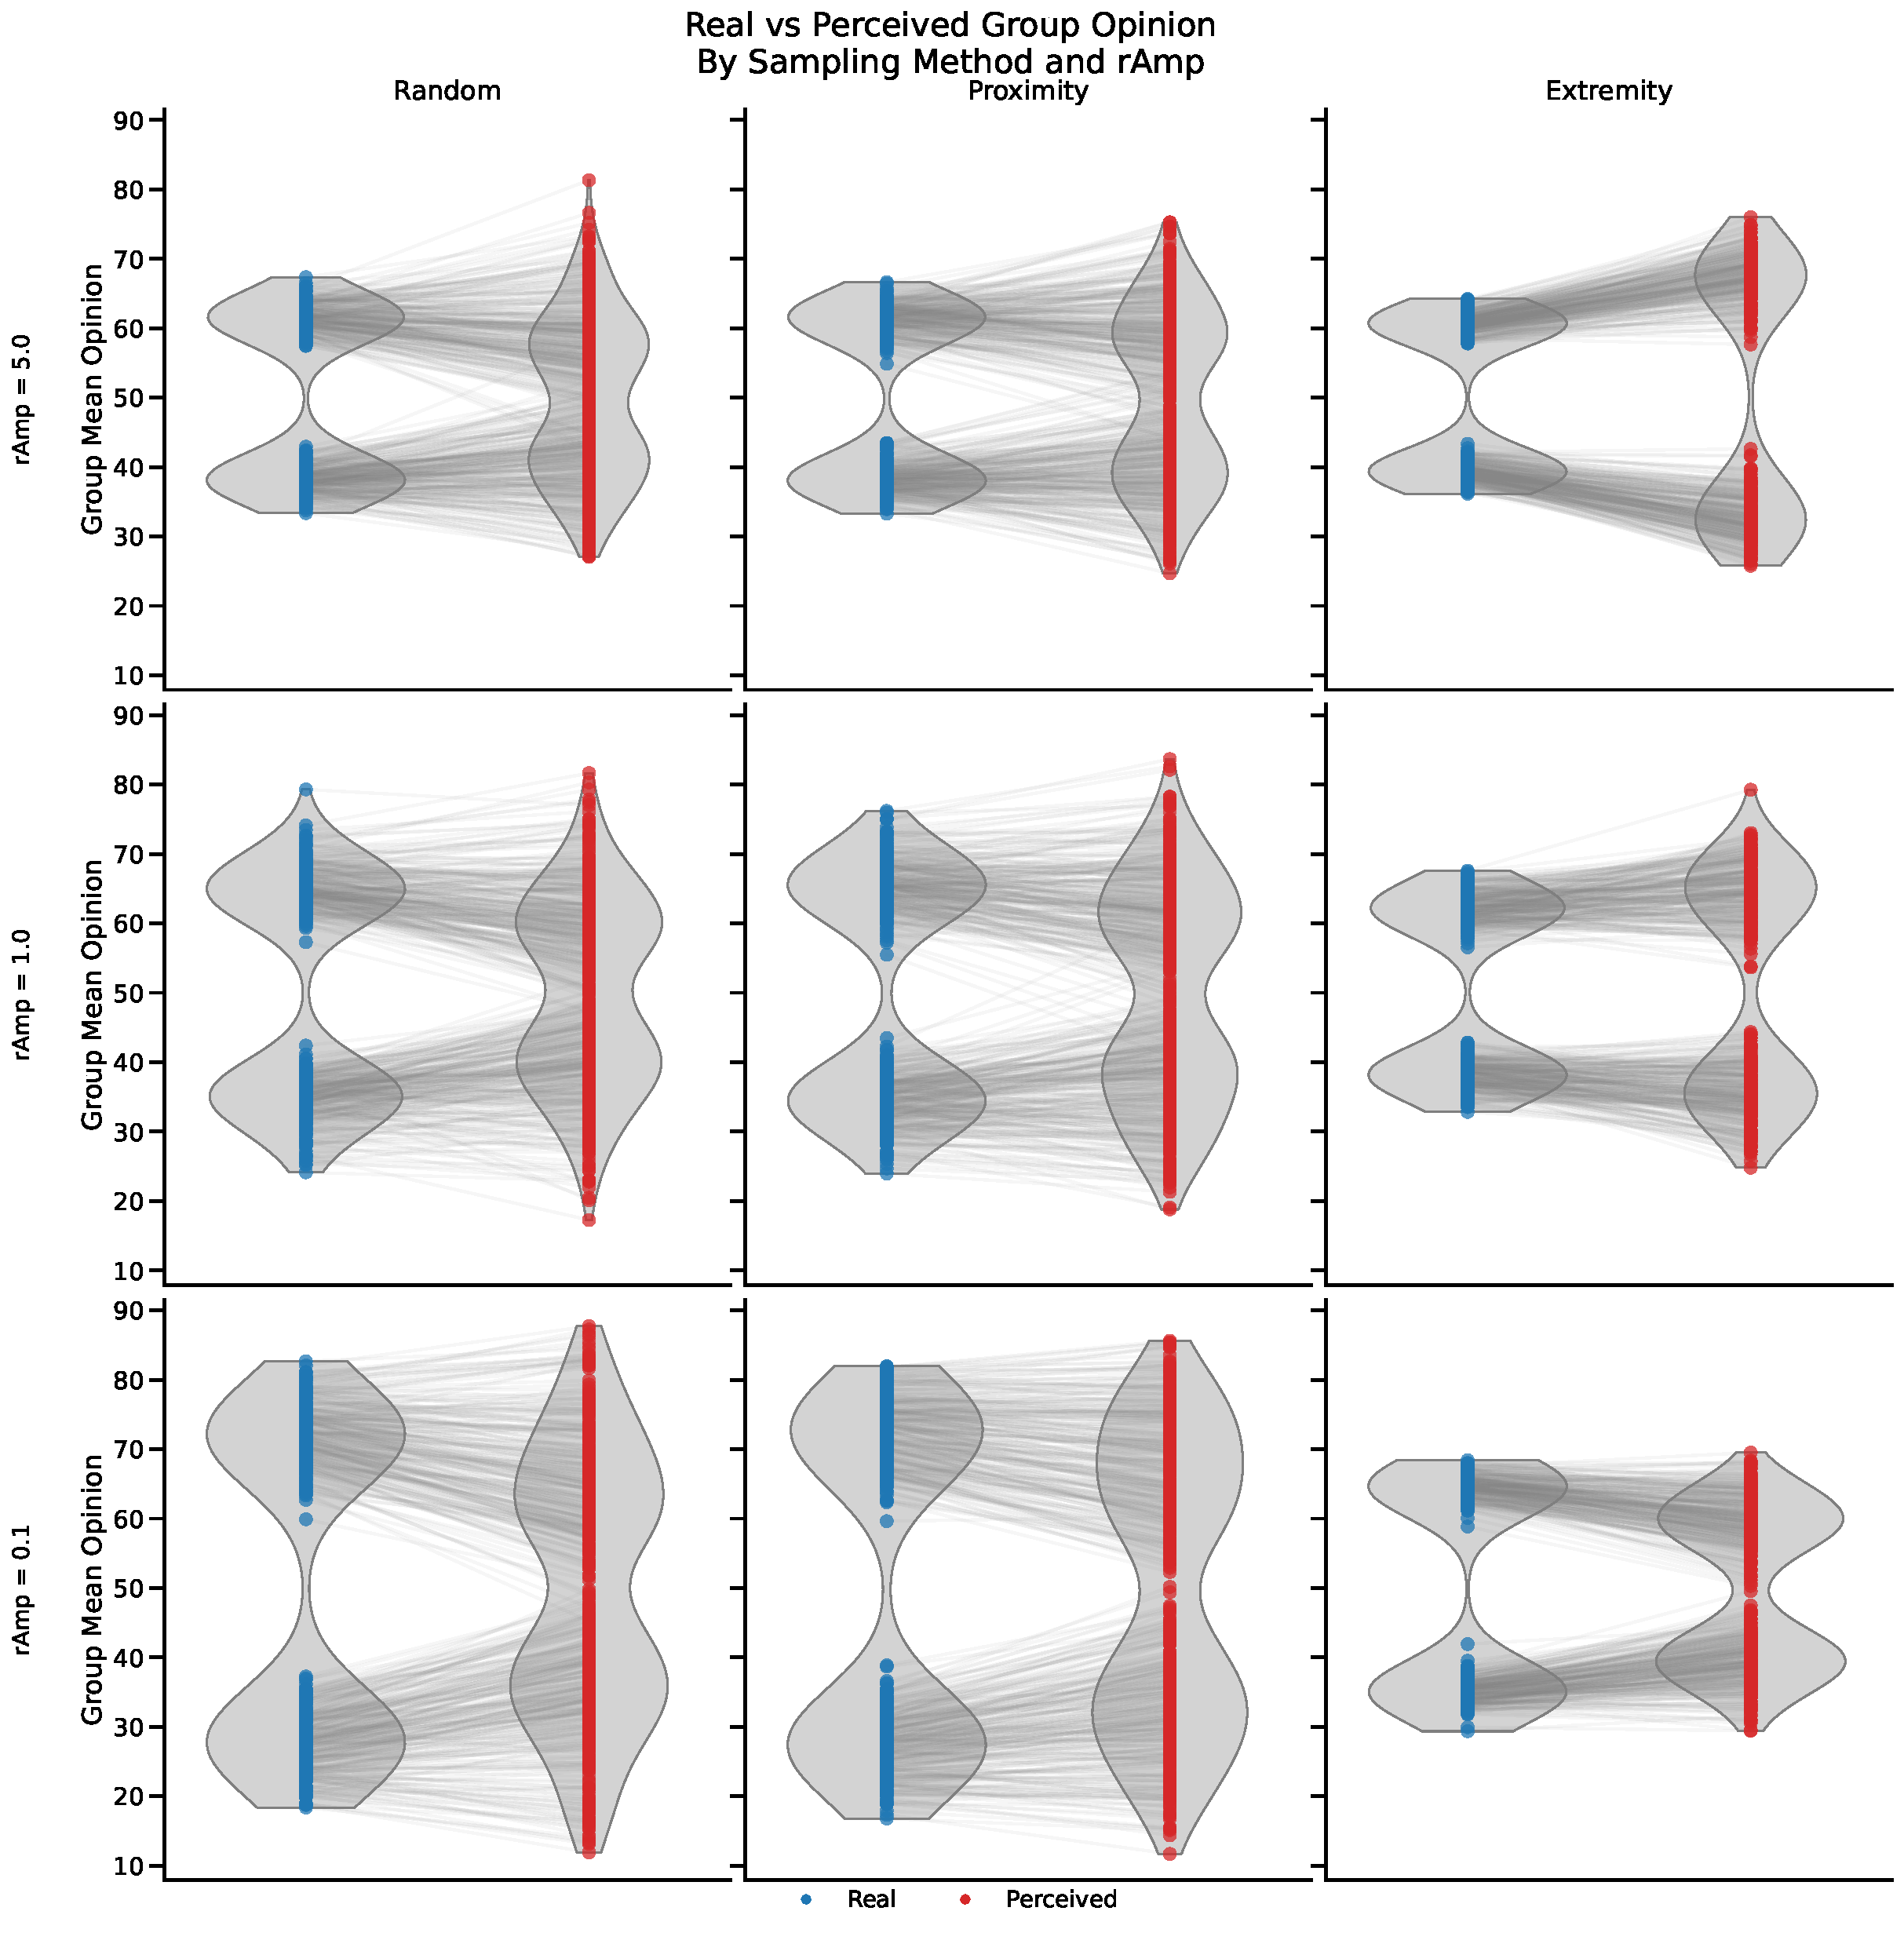
\includegraphics[width=1.0\textwidth]{images/figure1_3x3_v6.pdf}
  \caption{
    Real vs perceived group opinion means by sampling type and Repulsion learning rate (250 simulations each). Each point represents either the real or perceived group opinion mean within a single simulation; lines connect real and perceived group opinion means for each simulation. Violin plots show distributions for real and perceived means. 
}
~\label{fig:s1_fig1}  
\end{figure}

We expected that extremity-biased sampling would produce false polarization regardless of repulsion conditions, but this was not the case. For extremity-biased sampling, lower $\gamma$ appears to produce clear false moderation; $\gamma = 1.0$ appears to produce accurate perceptions, and $\gamma = 5.0$ produces false polarization. The effect of the strength of repulsion to moderate false polarization was originally expected to occur under prototype-biased sampling, but prototype-biased sampling did not show this sensitivity to $\gamma$. 

Across all conditions, group means stabilize around approximately 40 and 60, indicating partial group sorting. Given a uniform distribution of agent true opinions, the idealized sorting configuration would suggest group means at around 25 and 75. 
% This dampened sorting suggests that some agents have not joined the idealized group by the time the simulations have stabilized. 

We then visualize false polarization by plotting the signed discrepancy statistic for ingroup perceptions, $\Delta_g$, in a scatterplot. This allows us to achieve a better understanding of the differences between sampling methods as they vary with $\gamma$. Fig.~\ref{fig:s1_500sims_sampling_scatter} shows the false polarization scatter plot for all simulations.

\begin{figure}[htbp]
  \centering
  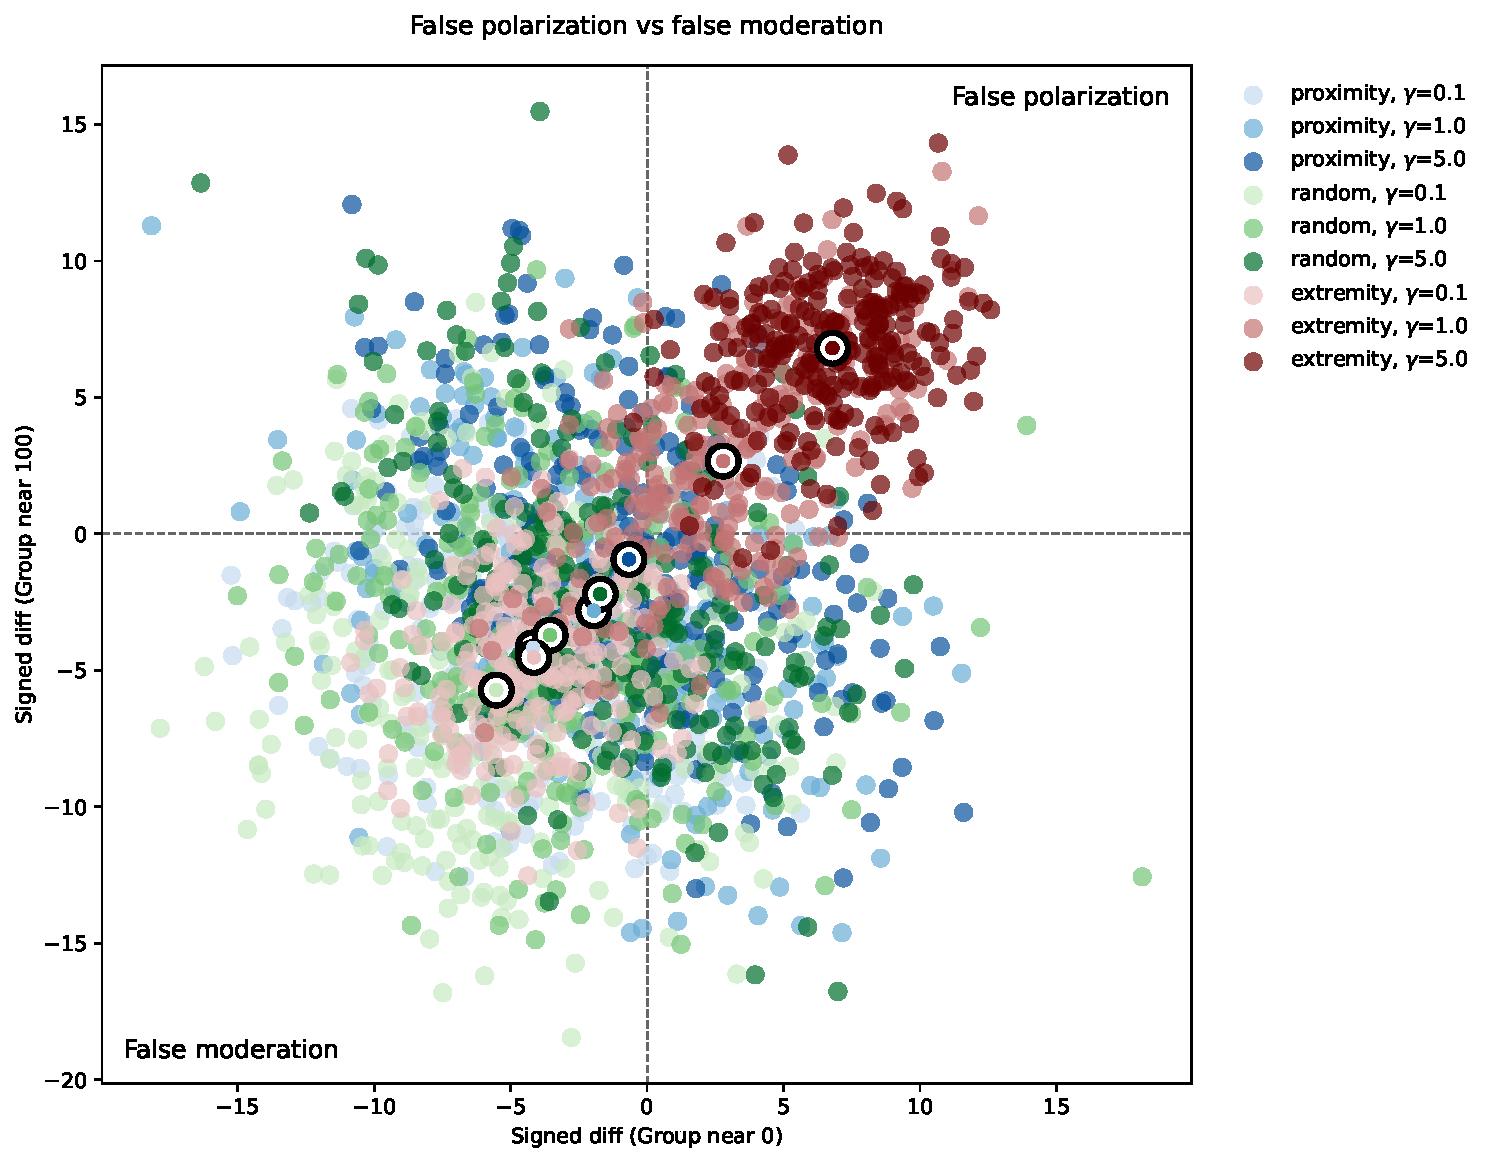
\includegraphics[width=1.0\textwidth]{images/falsepol_scatter_v2.pdf}
  \caption{
    Scatter plot of the signed discrepancy, $\Delta_g$, by group. Groups have been relabeled to their nearest poles to ensure simulations above and below the diagonal are interpretable. 250 simulations are plotted per parameter combination; points with open black borders denote simulation means across sampling type and $\gamma$. Quadrants of the plot correspond to qualitatively different intergroup misperceptions. Quadrant I corresponds to equal false polarization in both groups, Quadrant III corresponds to equal false moderation, and the remaining quadrants capture asymmetric cases in which one group is more accurate while the other is more inaccurate. 
}
~\label{fig:s1_500sims_sampling_scatter}  
\end{figure}

% Expand
There was a trend towards false polarization with higher $\gamma$ which aligns with expectation that a greater repulsion force would push groups further away from each other, but this is only strong in the case of extremity-biased sampling. 
Extremity-biased sampling had an effect where groups were more likely to be aligned in their relative perceptions of themselves compared to other sampling methods. That is, if one group perceived themselves to be closer to their nearest opinion pole, then the other group also perceived themselves to be closer to the other nearest opinion pole. 
For extremity-biased sampling, different values of $\gamma$ moderate whether the groups displayed false moderation or false polarization, while both groups remained aligned in how falsely moderated or polarized they were. 
Other sampling methods primarily showed either false moderation or an asymmetric pattern, and they showed a much wider and noisier spread of possibilities. Random and proximity-biased sampling showed a similar trend towards the first quadrant (upper right) as extremity-biased sampling, suggesting a trend towards false polarization, though most of these simulations do not express a $\Delta_g > 0$ for both groups. A number of simulations for both random and proximity-biased sampling show an asymmetric pattern of misperceptions, where one group's $\Delta_g$ is positive when the other's is negative. 

\subsection{Robustness tests}

% Discussing the parameters I tried
The pattern of results remained nearly unchanged across a range of parameter values. 
Varying the combinations of the following parameters did not substantially affect the magnitude or direction of group misperceptions across the following combinations of parameters: 
attraction rate $\alpha \in {0.1, 0.2, 0.4}$, repulsion rate $\gamma \in {0.3, 1.0, 3.0} $, group sample size $(ingroup, outgroup) \in {(100,100), (100,50)}$, and sensitivity parameters $\beta = \eta = 2.0$ or $\beta = \eta = 4.0$. 
% ADD OTHER PARAMETERS HERE
Extremity-biased sampling showed less sensitivity to varying $\gamma$ when $\alpha$ was either higher or lower than $\alpha = 0.2$, and it was the only sampling method to show sensitivity to parameterization.
This suggests that the observed dynamics are not sensitive to learning rate parameters within a broad range, and that the absence of strong misperception effects is not driven by specific parameter choices.

Significant qualitative changes emerged in the model when varying the way that group perceptions were initialized. We tested perception initialization methods to ascertain whether model dynamics led to the expected group sorting. Depending on how group perceptions are initialized, agents will have a different degree of consensus about the decision boundary between the two groups from the start of the simulation. 
%These tests determine how well the system is able to achieve consensus in perceptions. 
Because agents decide on groups to join solely based on their perception values, a consensus of which group to join should evolve from system dynamics above random chance. 
These tests determine how well the system dynamics are able to drive any kind of consensus in agent's perceptions to suggest that agents are sorting themselves, and not just randomly placing themselves, into groups. 
In the first test, perceptions were initialized as uniformly random, representing a complete lack of initial consensus; in the second test, perceptions were initialized as the true means of each group at $t=0$, representing complete consensus about groups. 
These two extreme cases are compared to the method used in the main results where perceptions of groups are initialized as separate Gaussian distributions with overlap and some consensus and some dissensus exists, representing a middle-ground approach to model initialization. 

When perceptions were initialized randomly, the model did not produce expected temporal dynamics (example plots, Figure~\ref{fig:s1_sim_example_sampling_initrand}). Group true opinions and perceptions stayed roughly constant throughout simulations, regardless of sampling method. This suggests that the system's dynamics were largely unable to dynamically arise, and that the system is surprisingly robust to noise acting as a seed for dynamics. 

\begin{figure}[htbp]
  \centering
  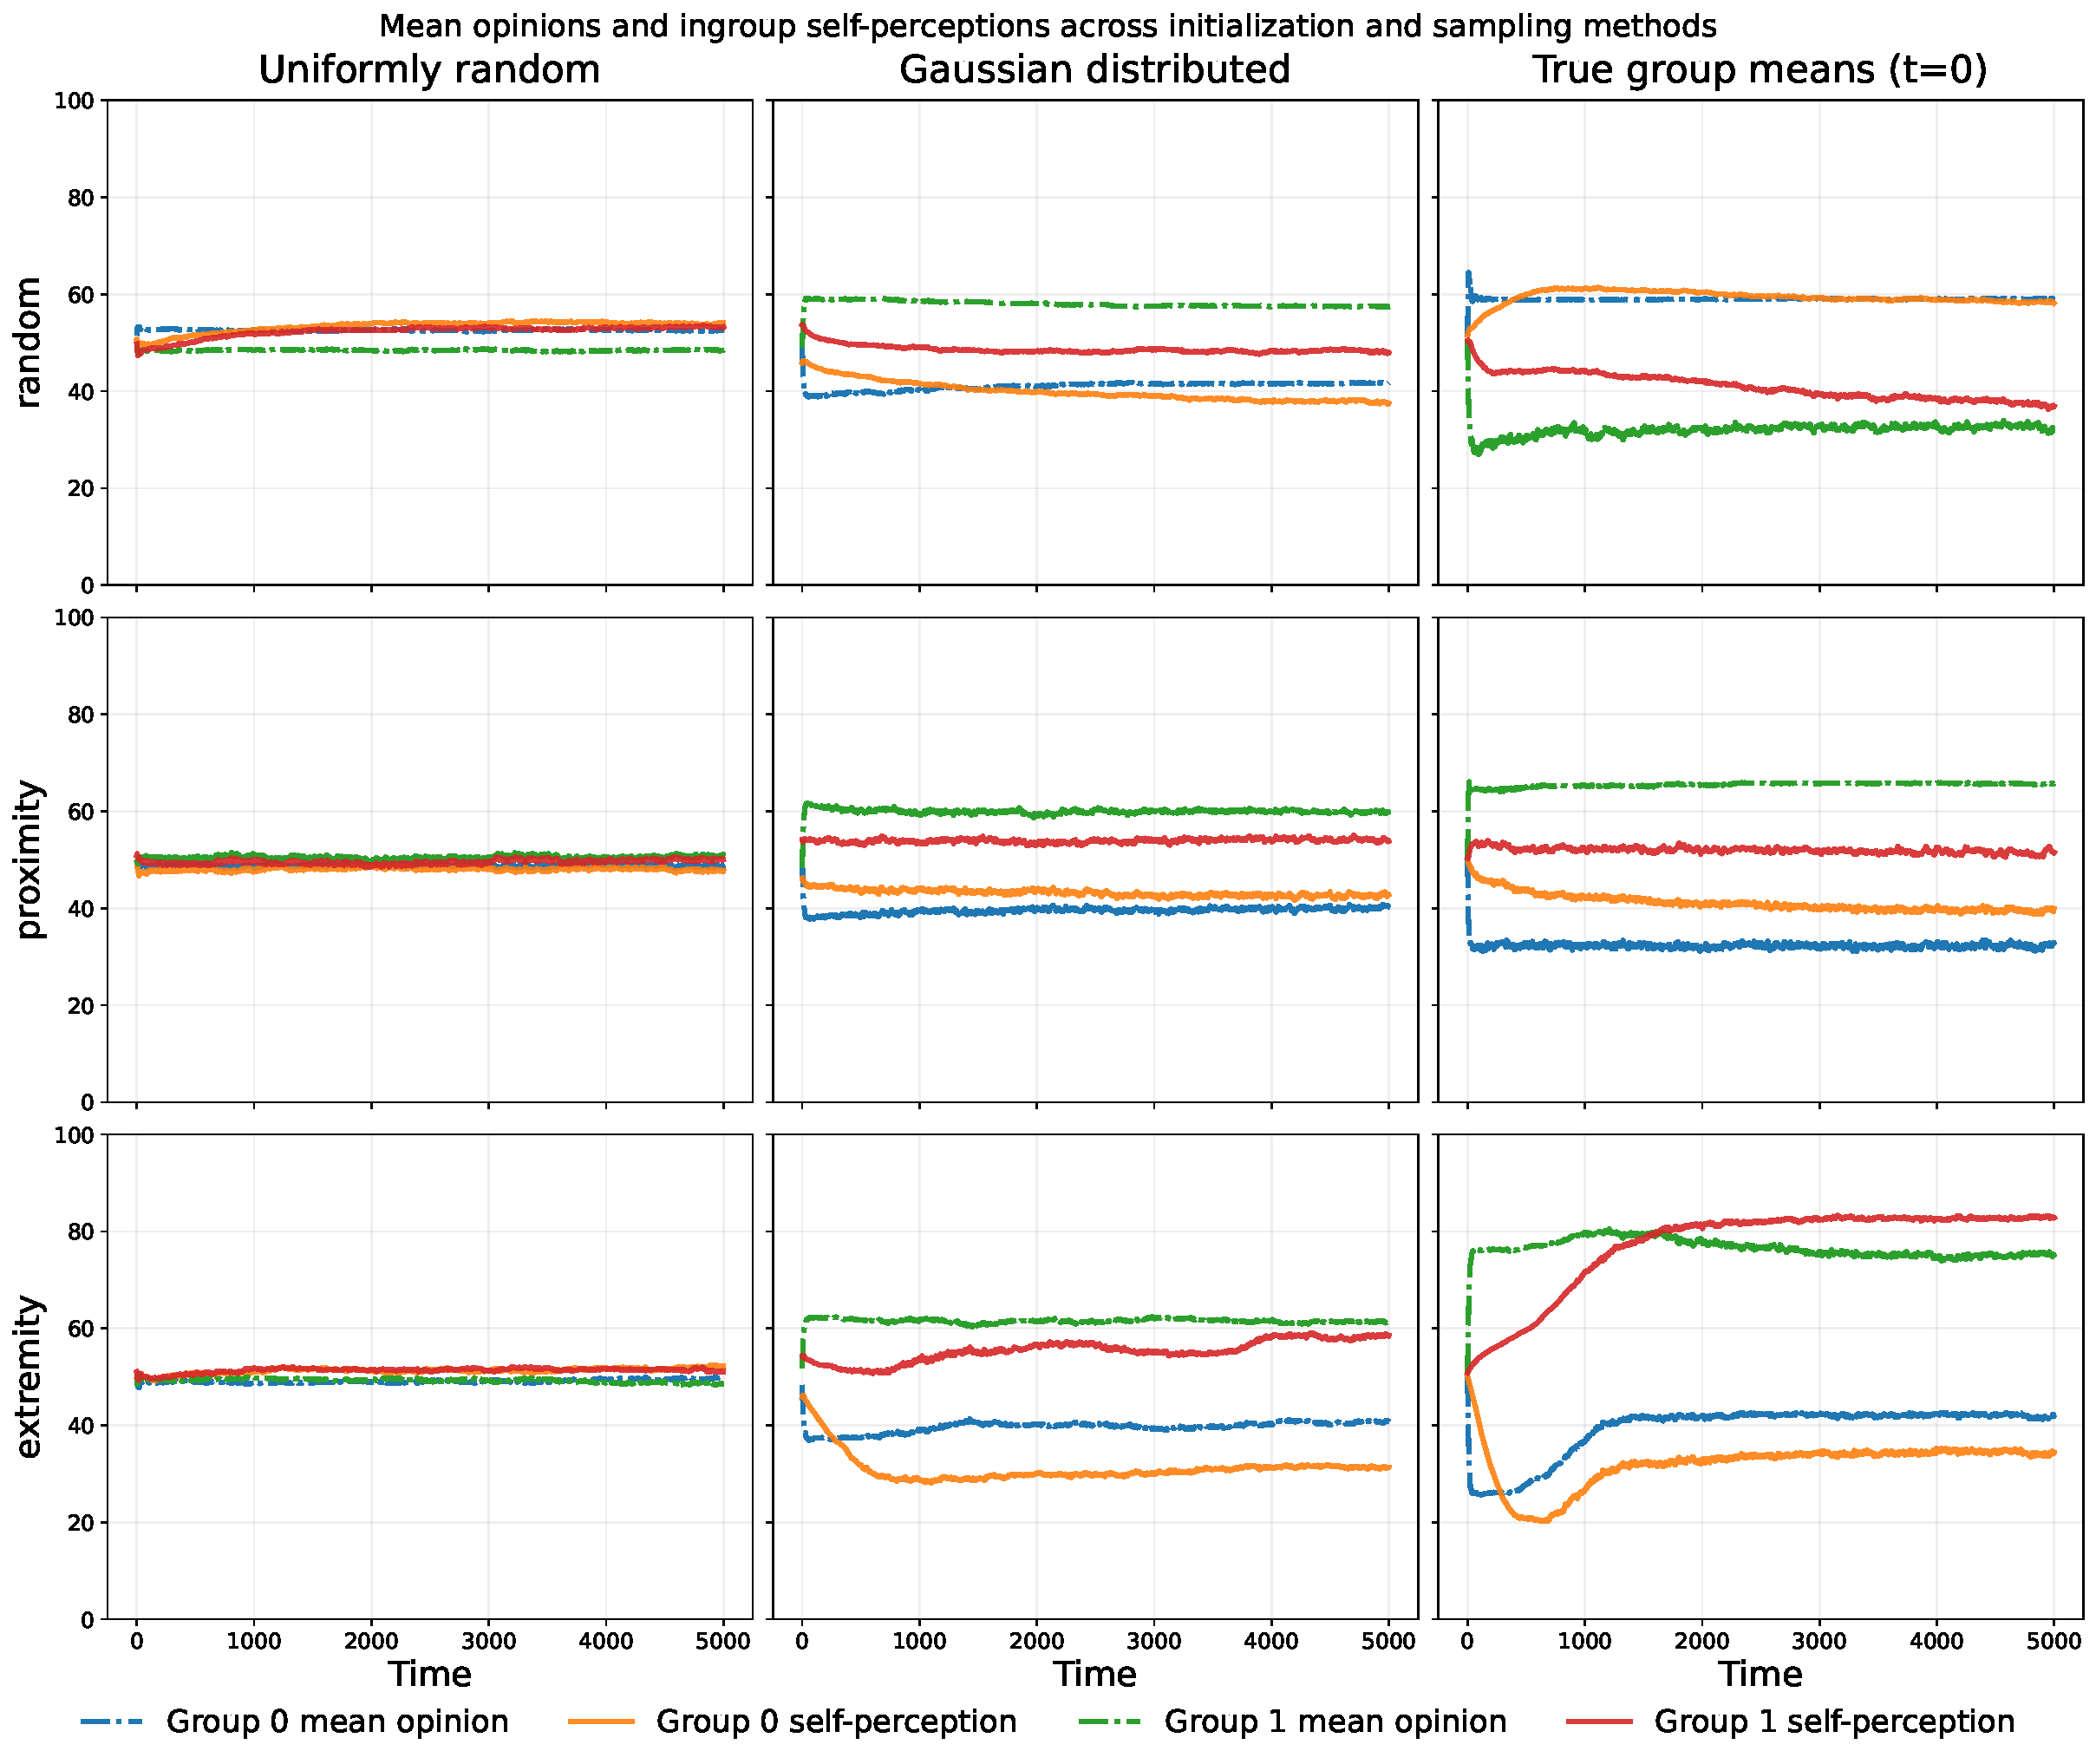
\includegraphics[width=1.0\textwidth]{images/robustness_singlesims_v1.pdf}
  \caption{
    Single simulation plots of mean real and perceived group opinions over time, varying perception initialization method and sampling type. Qualitative differences in dynamics are clear across perception initialization methods, showing a sensitivity to initial conditions. All other parameters were held constant between simulations: $\alpha = 0.4$, $\gamma = 1.0$, $\beta = \eta = 2.0$. 
}
~\label{fig:s1_sim_example_sampling_initrand}  
\end{figure}

%A test of 500 simulations per sampling type visualizing the pole-oriented signed discrepancy statistic ( $\Delta_g$ ) shows even variation and no effect between sampling types (Fig.~\ref{fig:s1_500sims_initrand}). 
% \begin{figure}[htbp]
%   \centering
%   \includegraphics[width=1.0\textwidth]{images/diss_groupshift_500sims_initrand.png}
%   \caption{
%     500 simulations per sampling type. Parameters: $\beta = 1.0$, $\eta = 1.0$, $\alpha = 1.0$, $\gamma = 1.0$.
% }
% ~\label{fig:s1_500sims_initrand}  
% \end{figure}

% RESUME EDITING HERE
When perceptions were initialized as the true means of the groups at $t=0$, the system produced more drastic dynamics of group sorting. Agents appear to rapidly sort into groups, and perceptions update more slowly to catch up to the rapid changes in true group means. Group means stabilize to values with greater differences than for either of the other initialization methods. When we consider how these alternate initialization tests affected group mean dynamics, the differences suggests that agents sort more efficiently depending on the clarity of the artificially introduced decision boundary at the beginning of the simulation. 

These qualitative differences in initialization methods suggest that the model dynamics for group sorting may be complicated by perceptions as an information layer. The model may be displaying dynamics more similar to cases where initial conditions quickly ossify perceptions and choices. An example of such a phenomenon occurs when students choose seats in a class on the very first day of a semester, and they each spontaneously retain the same seat throughout the semester. 


%====================================================
%  DISCUSSION
%====================================================

\section{Discussion}

In this model, we tested how social misperception arises when varying how individuals update their perceptions of groups using information from prototypical group members and their perceptions of other groups. 
We modeled a system where agents maintain individualized perceptions of group opinions and use those perceptions to voluntarily choose their group affiliation. Agents update their perceptions of group opinion toward members sampled from each group, and away from their perceptions of other groups, as inspired by Self-Categorization Theory (SCT, \cite{turner_rediscovering_1987}). We found that misperceptions do not appear to emerge easily when agents infer norms through gradual statistical learning. Across simulations, the population of agents perceived group opinion to align with mean group opinion on average. This was most consistent when prototypical group members were sampled via random sampling or proximity-biased sampling (sampling nearer the agent's perceptions). When prototypical group members were sampled via extremity-biased sampling (sampling nearer the poles), simulations showed some false polarization. Manipulating the strength of perception repulsion, following the meta-contrast principle, did not affect perception patterns for random and proximity-biased sampling. Extremity-biased sampling showed sensitivity to changes in repulsion strength, where lower repulsion strength led to false moderation and higher repulsion strength led to false polarization. Perceptions were more varied than real opinions across all conditions. 

Though the broad pattern was noise, some trends of misperceptions could be found. Across all sampling methods, increasing repulsion strength led to an increased tendency away from false moderation. The repulsion force was likely keeping group perceptions separated as $\gamma$ increased. 
Random and proximity-biased sampling methods tended towards false moderation with low repulsion strength when compared to extremity-biased sampling. Extremity-biased sampling showed a much tighter coupling of the discrepancy values, $\Delta_g$, calculated for each group. This implied that extremity-biased sampling not only tended to polarize groups, but it tended to do so evenly and symmetrically. 

Overall, the system showed robustness to misperceptions that contradicted the hypothesized effects. We hypothesized that proximity-biased sampling would show reasonable sensitivity to the combined attraction and repulsion effects, with random sampling indicating representative data of prototypical membership on average, and extremity-biased sampling showing clear false polarization. However, we found that random and proximity-biased sampling showed a general lack of misperceptions or false moderation, and extremity-biased sampling showed sensitivity to repulsion effects. 

\subsection{Lack of misperceptions}

% Why the lack of misperceptions?
We tested the system's sensitivity to initial conditions which may provide some insight into the model's mechanisms that explain the relative lack of emergent misperceptions. The model was particularly sensitive to the degree of initial consensus about the decision boundary between groups determined by the perception initialization process. 

% Point 1: Dampened sorting
The system showed significant sensitivity to initial perception conditions where other parameters had no effect. 
When initializing perceptions with perfect consensus about the group decision boundary, system dynamics were more drastic with greater changes in group means and perceptions. Meanwhile, when initializing perceptions completely randomly, groups did not appear to sort and system dynamics did not occur. Additionally, simulations appeared to sort early in the simulations, where the majority of group switching occurred at the beginning of the simulation. Changes in group perceptions evolved more slowly than group switching, and these changes in perceptions were not followed by significant changes in group switching. 
% ES: "It would be good to analyze switching in the simulation, and to show results in a graph."

%For a set of uniformly distributioned opinions between 0 and 100, the idealized sorting suggests that agents would sort into groups based on whether they were above or below 50, suggesting group means of 25 and 75. 
%In a robustness test where perceptions were initialized with a consensus about the decision boundary of which group to join, the system settles to these values. 
%In the primary results, where perceptions were initialized to be noisy but with an underlying difference in distributions, the system exhibits dampened sorting 
%When perceptions are initialized as uniformly random, the system is surprisingly robust to change and system dynamics do not evolve. 

% Point 2: Most sorting happens early
%Most membership sorting occurs early in the simulations. When reviewing single simulations, the majority of switching groups appears to occur at the beginning of the simulation. 

% Explaining need for structured perceptions
This suggests that the model may require some structure in perceptions for the mechanisms to drive dynamics, and this structure in perceptions may not be evolving from the update rules alone. The agent process can be conceptualized as a learning process where agents update 2 parameters to estimate a single decision boundary distinguishing two choices. This may be a nontrivial task, even when sampling relatively large ($\delta = 100$) group samples. When perceptions, group affiliations, and agent opinions are all initialized uniformly randomly, the agent is effectively tasked to use two slow-updating parameters to learn to distinguish two statistically identical distributions. Since agents are not able to do this, they sort themselves based on their random personal perceptions, which leads to random, rather than structured, group sorting. Initializing perceptions with some structure, as in the main results, provides some structure for agents' learning process to guess. However, the non-ideal group sorting may suggest that this process is partial, where some agents are able to update their perception parameters to learn to distinguish the groups and join the group closest to them, and other agents retain values closer to their initialized perceptions and fail to join the group closest to them.  

% How it plays through in the model
If agents are largely sorting based on their initialized perception values, then perception dynamics may be impeding, rather than driving, system dynamics. 
Single simulation runs appear to indicate that perception updating is a slow process relative to group change. 
The slow and incremental updating process may be coupling with the repulsion force to prevent agents from adapting their perceptions. 
For example, if an agent originally saw groups as being flipped relative to their true opinions, it's possible that the Repulsion force prevents agents from inverting their perceptions by negating the effects of contrary evidence. 
Additionally, the exponential kernel of the Attraction force acts as a confirmation bias that further suppresses any effect of observations which could help them flip this relationship. 
These may also contribute to possible subgroups of agents that are not able to align their perceptions with reality. 

% Overarching intuition
The competing perception updating mechanisms may be preventing individual agents from voluntarily associating into groups closer to an ideal configuration. 
Independently, attraction and repulsion forces on their own help agents update their perceptions to correspond with groups' true means, which creates a feedback loop that promotes agents to sort into separate groups based on their opinion values. However, when competing perception mechanisms are applied simultaneously, they inhibited group sorting. Perception repulsion pushed any individual agent's perceptions away from each other, likely increasing the amount of contrary evidence the agent needed to suggest a group switch. Though perception attraction would normally help to promote group differentiation, here it kept agents' perceptions anchored to the current group configuration. As a result, the perception rules prevented the system from evolving its own sorting configuration, and the system became more sensitive to initial conditions. This contradicts the intuition that more forces pushing people into groups would lead to greater sorting and thus greater polarization. 

% Major contributor: exponential kernel
The exponential kernel of the perception updating mechanism may also be contributing to the relatively slow updating process. 
The exponential kernel is intended to capture the psychological tendency to discount outliers from affecting perceptions of groups, as a kind of confirmation bias. The proximity-biased sampling serves as an additional layer of confirmatory tendency to see opinions in the world similar to one's own. 
Even the effects of extremity-biased sampling method are punished because extreme opinions (from one's own perceptions) are localized to only influence those with nearby perceptions of group opinion. 
It is possible that the extremity-biased sampling did not exhibit greater false polarization due to the heavy dampening effect of this kernel. 
Existing models of group sorting suggest that confirmation biases themselves lead to polarization, particularly when agents share opinions directly (\cite{hegselmann_opinion_2005}). 
% Hegselmann & Krause (2002)
This model could suggest that when those rules are used to update perception-mediated decision making rather than decisions based on personal opinions, they may serve to dampen rather than amplify those effects. 

% Implications for meta-contrast principle as a mechanism
% One possible mechanical outcome of the repulsion effect, and the meta-contrast principle in general, may be that it prevents individuals with these flipped perceptions from righting their perceptions with data. 

% Theoretical implications --------------------------------------------

\subsection{Theoretical implications}

% The model, on perception effects and misperceptions
These outcomes point to the possibility that inference of group opinion from even biased samples may not produce significant group-level misperceptions alone. 
It is possible that perception-mediated actions can be more robust to polarization dynamics than expected. In other agent-based models where numerical values representing group opinions or norms are public knowledge and communally modified, minor deviations substantively change any decisions for agents whose choices rely on those values. In this model, there is a mediating layer of perceptions which need to be altered by model dynamics in order to provide sufficient signal to agents to meaningfully act. If effects on perceptions are filtered through confirmation bias, it may be unlikely for agents to change their minds when observing other's opinions even when they differ significantly from the agent's expectations of the associated group. 
When data is used to update perceptions rather than opinions directly, the model may show that a confirmation bias that discredits distant data cancels out a sampling process that targets extremes to some extent. 

% Other work showing the effects of sampling
Misperceptions may not robustly occur in domains where actions are mediated through group perceptions as a mechanism, unless the space of perceptions is structured to facilitate decisionmaking. 
Some existing agent-based models which incorporate SCT have shown that clusters of opinions separate and form when driven by opinion updating rules implementing the meta-contrast principle (\cite{salzarulo_continuous_2006}), 
% Laurent Salzarulo (2006)
but the model differs by having agents adapt their own personal opinions to information. 
Social sampling has been found to be a significant driver of differential social judgments on its own, including group misperceptions (\cite{galesic_sampling_2018}). 
% Galesic, M., Olsson, H., & Rieskamp, J. (2018). A sampling model of social judgment.Psychological Review, 125(3), 363–390. https://doi.org/10.1037/rev0000096
However, this model suggests that such sampling may not lead to widespread configurational misperceptions in the context of other perception effects. 

% The model, on sorting
If unsorted members persist in the model, this suggests an area of social misperception at the individual level that corroborates extant concerns about misperception measurement. 
The contribution of subgroup misperceptions to pluralistic ignorance has been proposed, particularly as a methodological concern for measurement. 
(\cite{segrist_yeah_2007}) found pluralistic ignorance of drinking norms among high schoolers, but they noted that nondrinkers exhibited the most misestimation of the high school's norms. They note that surveying drinkers alone may not have reached the same conclusion. 
% Segrist et al 2007
They suggested that this may constitute a measurement error; although the referent population for the survey was the high school in question, they argued that the difference between drinkers and nondrinkers was a significant alternate axis that led to the inclusion of outgroup members into perceptions of ingroup behavior. 
Contributions of subgroups may be difficult to assess because pluralistic ignorance is not well defined across group scales. 
Further investigation into unsorted members in the model is needed to determine how they contribute to misperceptions. 

% Contribution of the model to SIT/SCT theory
% ES: "SIT/SCT mostly assumes relatively unchangeable group identities. I'm not sure how much of that line of theory applies when switching is easy. But probably the predictions you make (prototype-based perceptions of groups, metacontrast) would hold. But other predictions, especially regarding ingroup-outgroup asymmetries, might not hold when switching is trivially easy."
One limitation of this work is that this model implements a particular operationalization of Self-Categorization Theory principles where group switching is technically trivially easy. 
This may not correspond with real-world groups where institutional, relational, or biographical constraints increase the barrier to group switching. 
SCT perception processes may occur as people attempt to negotiate their self-identity and status in group membership they otherwise cannot change. 
Prior work has found that the ease of group switching affects how people perceive their identification with the group (\cite{ellemers_influence_1990}). 
% ??? CITE Ellemers, van Knippenberg, Wilke https://pubmed.ncbi.nlm.nih.gov/2224425/
This model finds that even when switching is formally easy, switching can become psychologically/dynamically difficult. 
This barrier can evolve out of the operationalized perception rules themselves. 

% Future work
Future work can incorporate known differences in ingroup and outgroup perception which could change a number of the model's simplifications. 
Currently, agents in the model sample equivalent members from both ingroups and outgroups; this could be changed to reflect known phenomena where people more likely encounter ingroup rather than outgroup members. 
The model may also show dampened effects due to the innate symmetries in the instantiation process: agent opinions are instantiated uniformly randomly, perceptions are instantiated evenly about the midpoint of the opinion scale, and the extremity-biased sampling method draws from both rather than one extreme. 
Instantiating the model with greater global asymmetry, such as initializing perceptions closer to one side of the spectrum than the other, could drive dynamics while reflecting real-world tendencies. 
Introducing these asymmetries may yield mechanistic pathways to greater group divisiveness that produces misperceptions. 
% PT: "what would happen if instead you selected views that are more distant from the individual i's views?  So this would be extremity-bias but only for those views that are more different from i's, which seems like it would fit with (and generate?) the meta-contrast effect..."
Lastly, model code naturally extends to more than two groups and more than one opinion dimension, so further work is needed to test how different values affect dynamics. 
Including multiple opinion dimensions can be used not only to represent alternate issue axes, but it can also be used to represent different modes known to affect group perceptions (e.g., human identity, social identity, and personal identity) (\cite{hornsey_social_2008}). 

One way that this model is distinct from other agent-based models of group sorting or polarization is that agent personal opinions remain fixed througout the simulation. 
This constraint was chosen to test whether changing perceptions causes misperceptions to emerge. 
When considering the outcomes of this model, future work may focus on systematically testing whether perception changes alone are necessary and sufficient for group misperceptions, and whether changes to personal opinion are a necessary component. 


\clearpage
% Only works cited in chapter01.tex appear here (no \nocite{*}).
\printbibliography[title={References}]
\end{document}
